\lecture{ANOVA}{ANOVA}
\section{Analysis of Variance Examples}

\title{Examples of Analysis of Variance}
\subtitle{Detecting a Difference Between Multiple Treatments}

%\author{Kelly Black}
%\institute{Clarkson University}
\date{3 April 2015}

\begin{frame}
  \titlepage
\end{frame}

\begin{frame}
  \frametitle{Outline}
  \tableofcontents[hideothersubsections,sectionstyle=show/hide]
\end{frame}



\subsection{Example}

\begin{frame}{Time in Bankruptcy}

  When a firm is in a financial crisis there are many options. One
  option is to declare some form of bankruptcy to get relief from
  creditors. There are many ways to proceed in bankruptcy. We look at
  three types of plans for getting out of bankruptcy: No Prefiling (N),
  Prepackaged (P), and Joint Exchange (J).

  \vfill

  A number of firms were sampled at random, and their plan as well as
  time in bankruptcy (in weeks) were sampled.

  \vfill
  Question: Is there a difference?

  
\end{frame}

\begin{frame}{Time in Bankruptcy}

  A number of firms were sampled at random, and their plan as well as
  time in bankruptcy (in weeks) were sampled.

  \vfill

  Question: Is there a difference?

  \vfill

  \begin{tabular}{rr|@{\hspace{2em}}rr|@{\hspace{2em}}rr|@{\hspace{2em}}rr}
    Plan & Time & Plan & Time & Plan & Time & Plan & Time \\ \hline
    N & 1.1 & P & 0.5 & N & 6.6 & N & 3.2 \\
    P & 2.5 & N & 5.0 & J & 5.2 & P & 3.5 \\
    J & 4.1 & P & 2.4 & J & 3.5 & P & 1.6 \\
    N & 6.2 & N & 3.1 & J & 2.2 & J & 3.0 \\
    J & 2.3 & J & 2.9 
  \end{tabular}

  
\end{frame}

\begin{frame}{Comparing Multiple Independent Samples}

  \only<2->{%
    \iftoggle{clicker}{%

      \redText{\textbf{Clicker Quiz: Is there a difference?}}

      \vfill

    }
  }

  \begin{columns}[t]
    \column{.33\textwidth}

      No Pre-Filing \\
      \begin{tabular}{l}
        1.1 \\ 6.6  \\ 3.2 \\ 5.0  \\ 6.2 \\ 3.1
      \end{tabular}


    \column{.33\textwidth}

      Pre-packaged \\
      \begin{tabular}{l}
        0.5 \\ 2.5 \\ 3.5 \\ 2.4 \\ 1.6
      \end{tabular}


    \column{.33\textwidth}

      Joint Exchange \\
      \begin{tabular}{l}
        5.2 \\ 4.1 \\ 3.5 \\ 2.2 \\ 3.0 \\ 2.3 \\ 2.9
      \end{tabular}


  \end{columns}

  \only<2->{%
    \iftoggle{clicker}{%

      \vspace*{-1em}
    
      \vfill

      \begin{tabular}{l@{\hspace{3em}}l@{\hspace{3em}}l@{\hspace{3em}}l}
        \redText{A: Yes}  & \redText{B: No} & \redText{C: Maybe}
      \end{tabular}

      \vfill
      \vfill
      \vfill
    }
  }


\end{frame}


\begin{frame}{Comparing Multiple Independent Samples}

  The point estimates:
    \only<1>{%
      \redText{No Pre-Filing}

      \begin{tabular}{rrrrr}
        Min. & 1st Qu. & Median  &  3rd Qu. &   Max. \\
        1.100 &  3.125 &  4.100  &   5.900  &  6.600 
      \end{tabular}

      \vfill

      \begin{tabular}{rr}
        Sample Mean & Sample Standard Deviation \\
        4.2 & 2.108
      \end{tabular}

      \vfill

      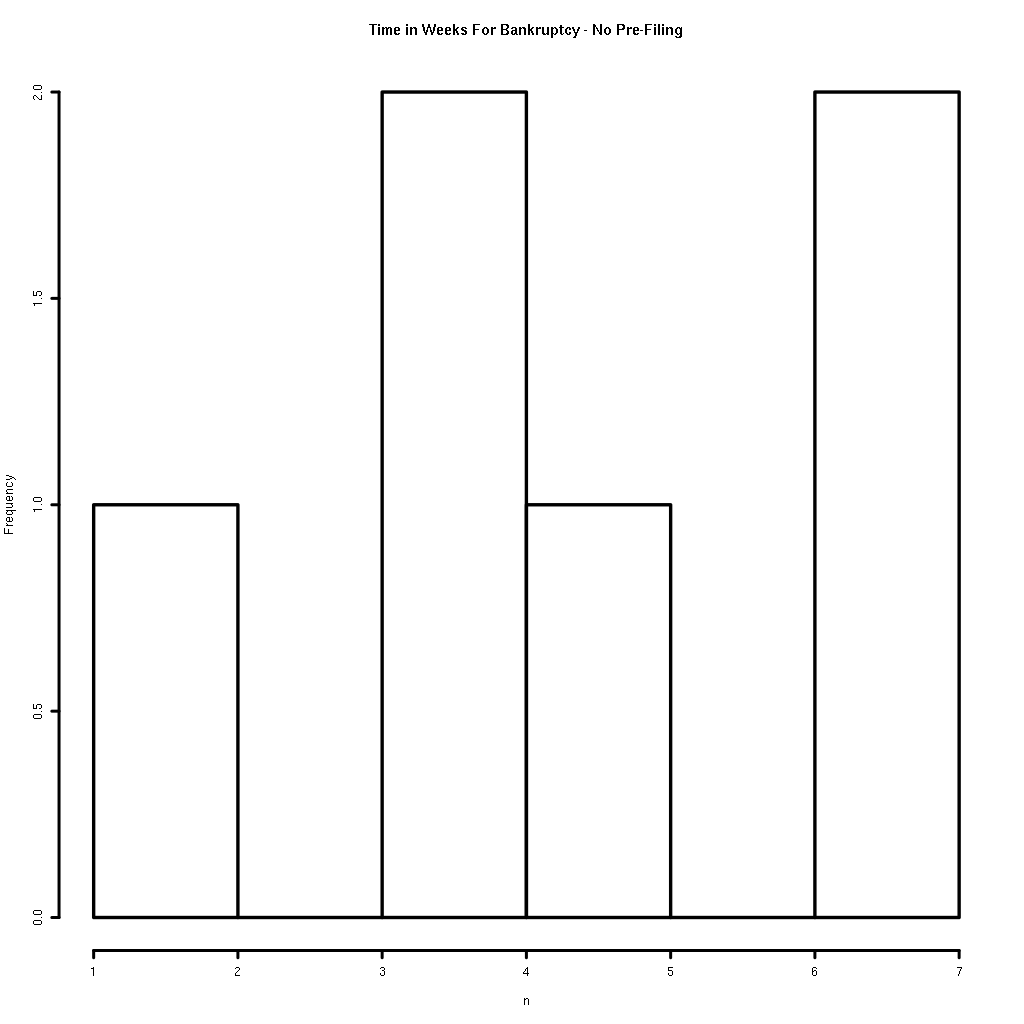
\includegraphics[width=4cm]{img/noPreFilingTime}
      
    }
    \only<2>{%
      \redText{Pre-packaged}

      \begin{tabular}{rrrrr}
        Min. & 1st Qu. & Median  &  3rd Qu. &   Max. \\
        0.5  &   1.6   &  2.4    &    2.5   &   3.5 
      \end{tabular}

      \vfill

      \begin{tabular}{rr}
        Sample Mean & Sample Standard Deviation \\
        2.1 & 1.120 
      \end{tabular}

      \vfill

      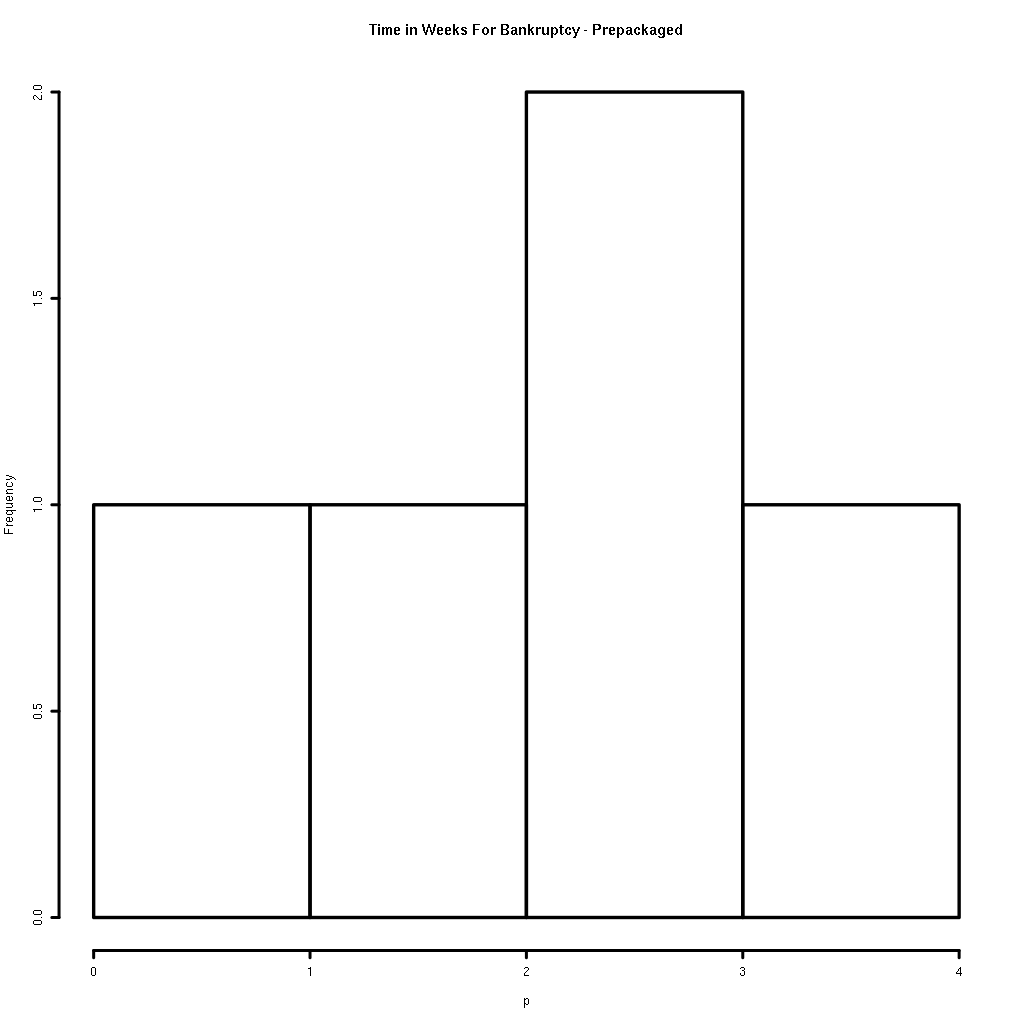
\includegraphics[width=4cm]{img/prePackagedTime}

    }
    \only<3>{%
      \redText{Joint Exchange}

      \begin{tabular}{rrrrr}
        Min. & 1st Qu. & Median  &  3rd Qu. &   Max. \\
        2.200 &   2.600 &  3.000 &   3.800  &  5.200 
      \end{tabular}

      \vfill

      \begin{tabular}{rr}
        Sample Mean & Sample Standard Deviation \\
        3.31 & 1.060
      \end{tabular}

      \vfill

      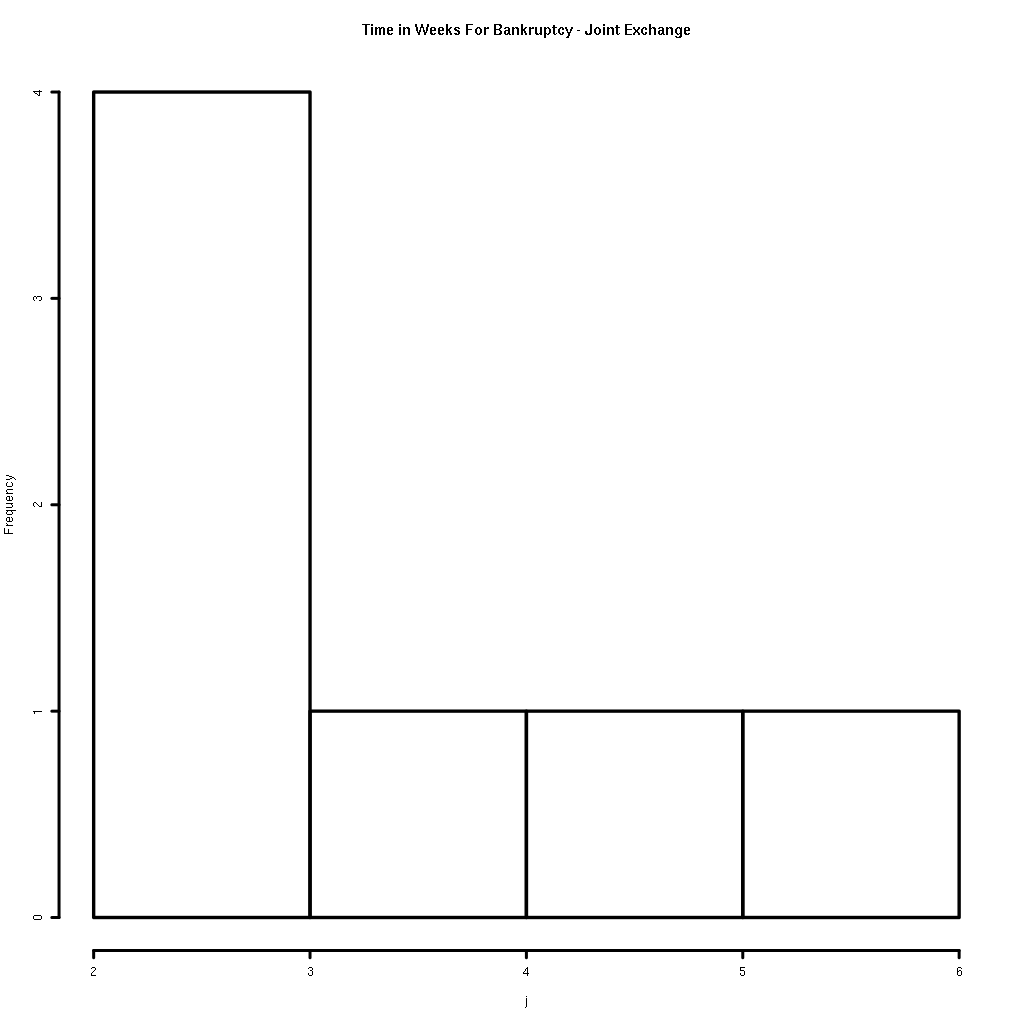
\includegraphics[width=4cm]{img/jointExchangeTime}

    }



\end{frame}

\begin{frame}{Conclusions?}

  Is there a difference?

  \vfill

  \begin{columns}[t]

    \column{.33\textwidth}

    No-Prefiling \\
    \begin{tabular}{rrr}
      $\bar{x}_1$ & $s_1$ & $n_1$ \\
      4.2 & 2.108 & 6
    \end{tabular}


    \column{.33\textwidth}

    Pre-Packaged \\
    \begin{tabular}{rrr}
      $\bar{x}_2$ & $s_2$ & $n_2$ \\
      2.1 & 1.120 & 5
    \end{tabular}


    \column{.33\textwidth}

    Joint Exchange
    \begin{tabular}{rrr}
      $\bar{x}_3$ & $s_3$ & $n_3$ \\
      3.31 & 1.060 & 7
    \end{tabular}


  \end{columns}

  \vfill

  \centerline{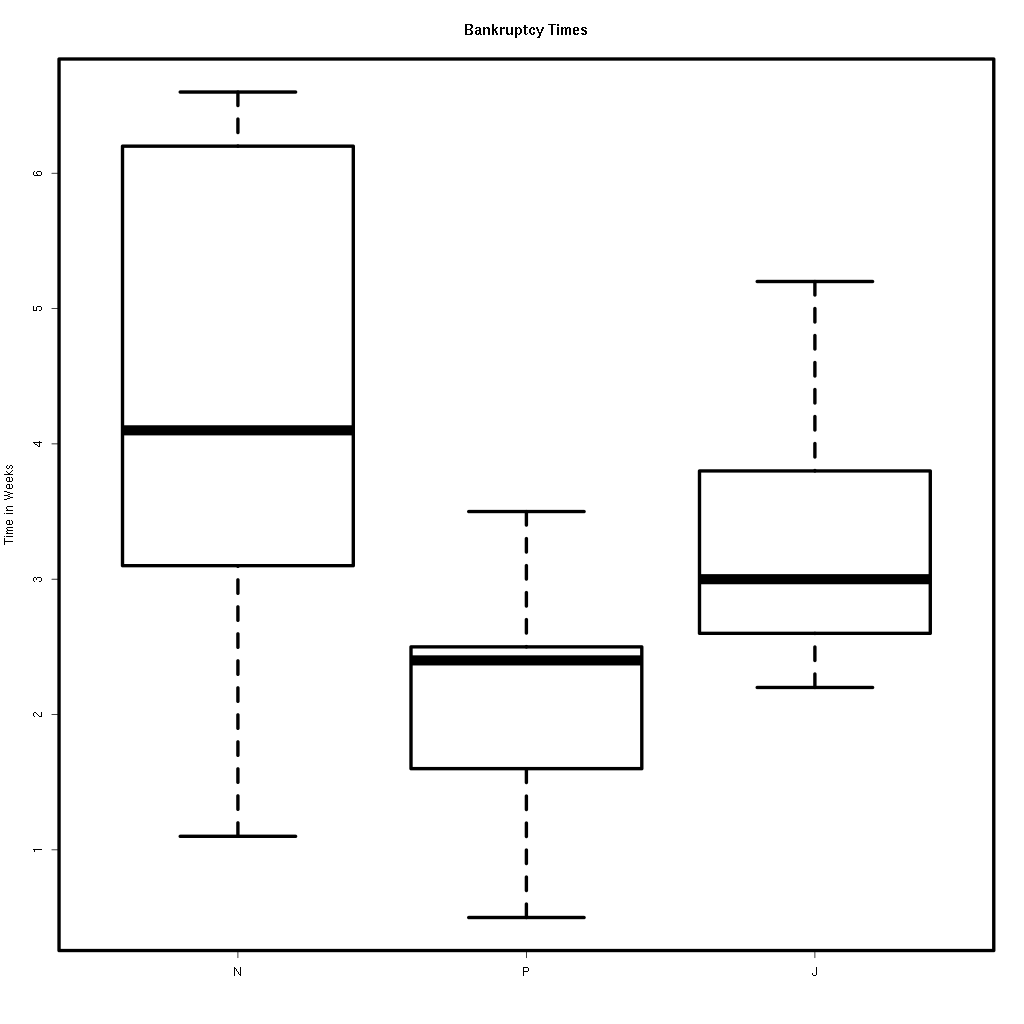
\includegraphics[width=4cm]{img/bankruptcyBoxplots}}

  \vfill

  How do we back up our claim?

  \vfill
  
\end{frame}

\subsection{Analysis of Variance}

\begin{frame}{Analysis of Variance}

  We have $k$ treatments and have measurements for each treatment. 


  \begin{eqnarray*}
    \begin{array}{lllll@{\hspace{3em}}rr}
      \mathrm{\color<1>{red}{Treatment~1:}} & \color<1>{red}{x_{1,1}}, & \color<1>{red}{x_{1,2}}, & \color<1>{red}{\ldots} & \color<1>{red}{x_{1,n_1}}, & \uncover<6->{ \blueText{\bar{x_1}} & \blueText{n_1} } \\ 
      \uncover<2->{\color<2>{red}{\mathrm{Treatment~2:}} & \color<2>{red}{x_{2,1}}, & \color<2>{red}{x_{2,2}}, & \color<2>{red}{\ldots} & \color<2>{red}{x_{2,n_2}}, & \uncover<6->{ \blueText{\bar{x_2}} & \blueText{n_2} } \\}
      \uncover<3->{\color<3>{red}{\mathrm{Treatment~3:}} & \color<3>{red}{x_{3,1}}, & \color<3>{red}{x_{3,2}}, & \color<3>{red}{\ldots} & \color<3>{red}{x_{3,n_3}}, & \uncover<6->{ \blueText{\bar{x_3}} & \blueText{n_3} } \\}
      \uncover<4->{\vdots  & \vdots  &       & \vdots \\}
      \uncover<5->{\color<5>{red}{\mathrm{Treatment~k:}} & \color<5>{red}{x_{k,1}}, & \color<5>{red}{x_{k,2}}, & \color<5>{red}{\ldots} & \color<5>{red}{x_{k,n_k}}. & \uncover<6->{ \blueText{\bar{x_k}} & \blueText{n_k} } }
    \end{array}
  \end{eqnarray*}

\end{frame}

\begin{frame}{Assumptions}

  \begin{eqnarray*}
    x_{i,j} & = & \mu_i + \sigma_{i,j}, \\
    \sigma_{i,j} & \thicksim & N(0,\sigma^2).
  \end{eqnarray*}

  \vfill

  We assume that all errors have the same variance!

  \vfill

  Hypothesis test:
  \begin{eqnarray*}
    H_0: & & \mu_1 = \mu_2 = \cdots = \mu_k, \\
    H_a: & & \mu_i \neq \mu_j ~\mathrm{for~some~}i,~j.
  \end{eqnarray*}

  \vfill
  
\end{frame}

\begin{frame}{Variance Away From What?}

  We have $k+1$ different point estimates for different means.
  \begin{eqnarray*}
    \bar{x}_1 & = & \frac{x_{1,1} + \cdots + x_{1,n_1}}{n_1}, \\
    \bar{x}_2 & = & \frac{x_{2,1} + \cdots + x_{2,n_2}}{n_2}, \\
              & \vdots & \\
    \bar{x}_k & = & \frac{x_{k,1} + \cdots + x_{k,n_k}}{n_k}, \\
    \bar{x}_T & = & \frac{n_1 \bar{x_1} + \cdots + n_k \bar{x_k}}{n_1+\cdots+n_k}, \\
    N_T       & = & n_1+n_2+\cdots+n_k.
  \end{eqnarray*}
  
\end{frame}

\begin{frame}{Three Measures of Variation}

  % x_{tr} \approx 3.272222

  We have three measures of variance: \\
  \begin{tabular}{ll}
    SSTr & $=$ \\ % 12.04754
    SSE  & $=$ \\ % 33.98857
    SST  & $=$ \\ % 46.03611
  \end{tabular}
  
\end{frame}

\begin{frame}{Interpretation}

  Hypothesis test:
  \begin{eqnarray*}
    H_0: & & \mu_1 = \mu_2 = \cdots = \mu_k, \\
    H_a: & & \mu_i \neq \mu_j ~\mathrm{for~some~}i,~j.
  \end{eqnarray*}

  \only<1>{\centerline{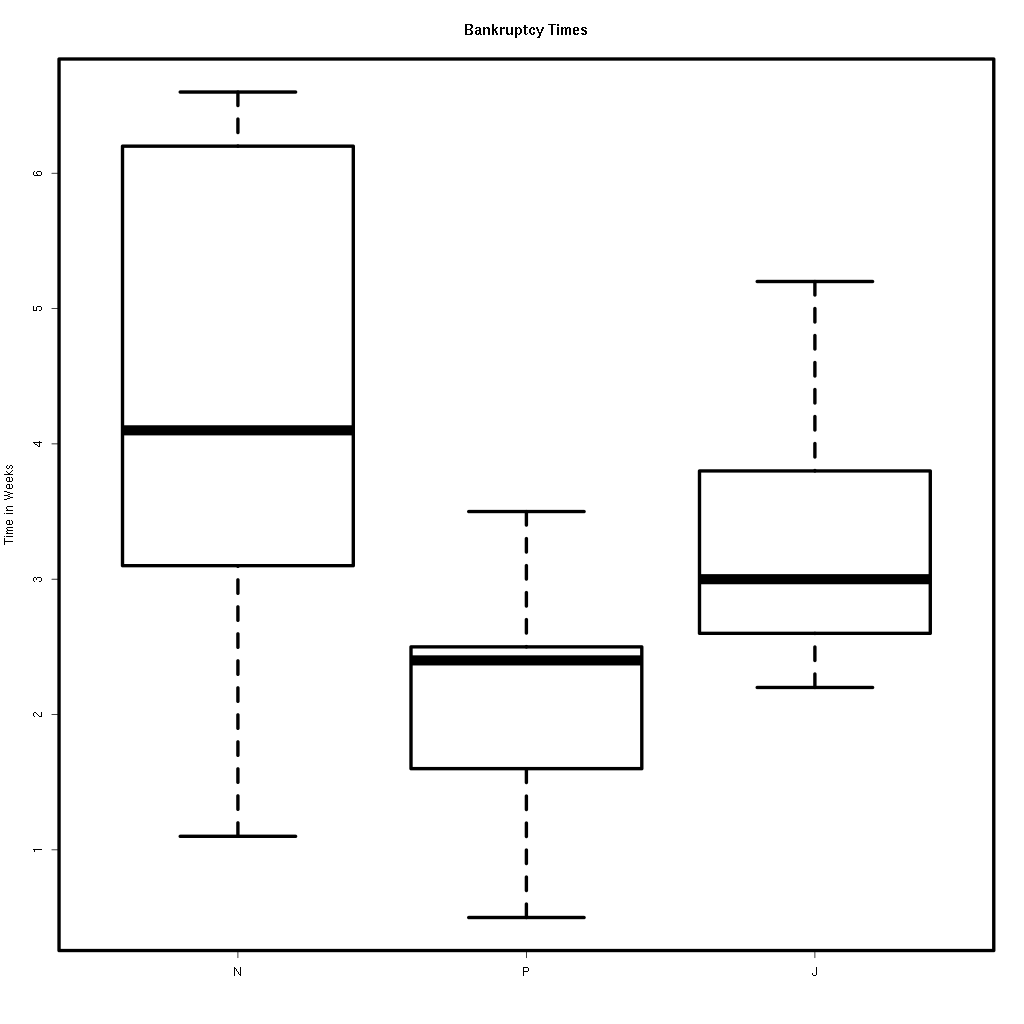
\includegraphics[width=4cm]{img/bankruptcyBoxplots}}}
  \only<2>{\centerline{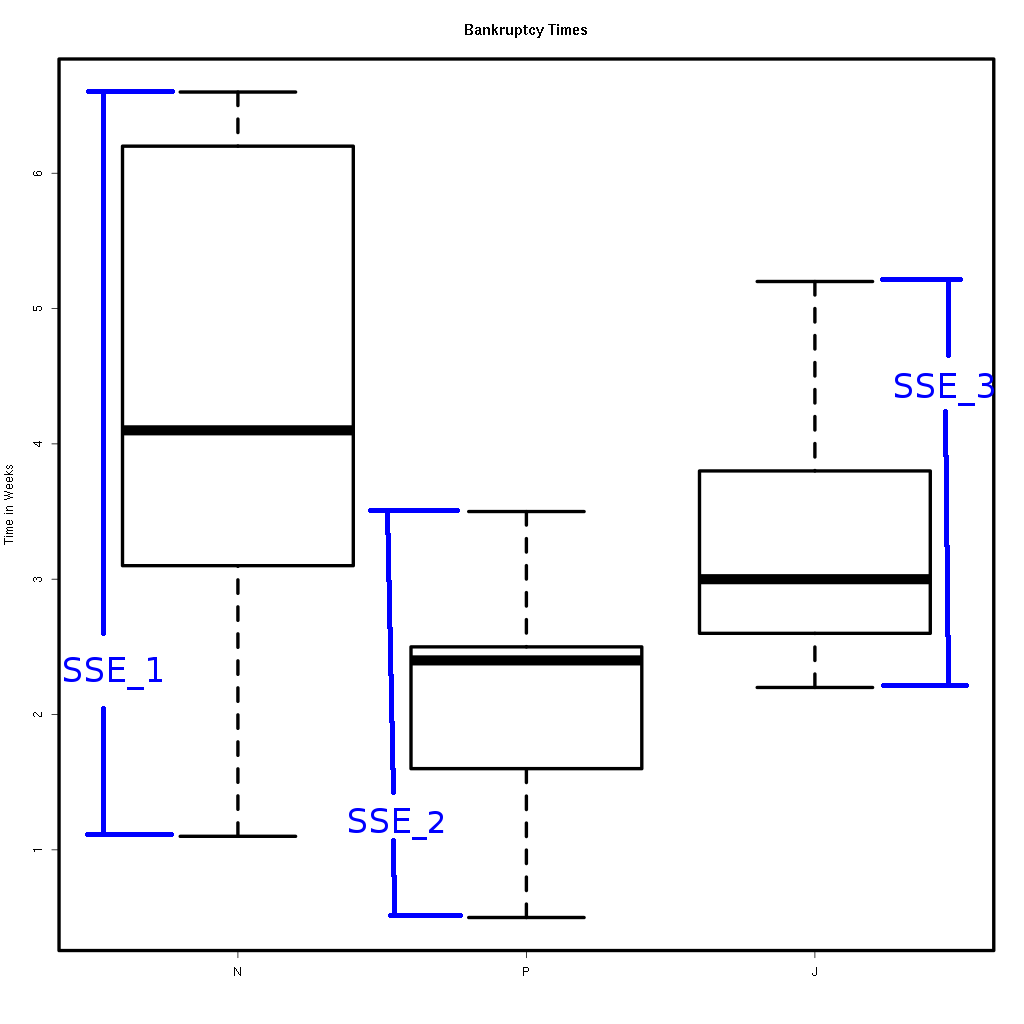
\includegraphics[width=4cm]{img/bankruptcyBoxplotSSE}}}
  \only<3>{\centerline{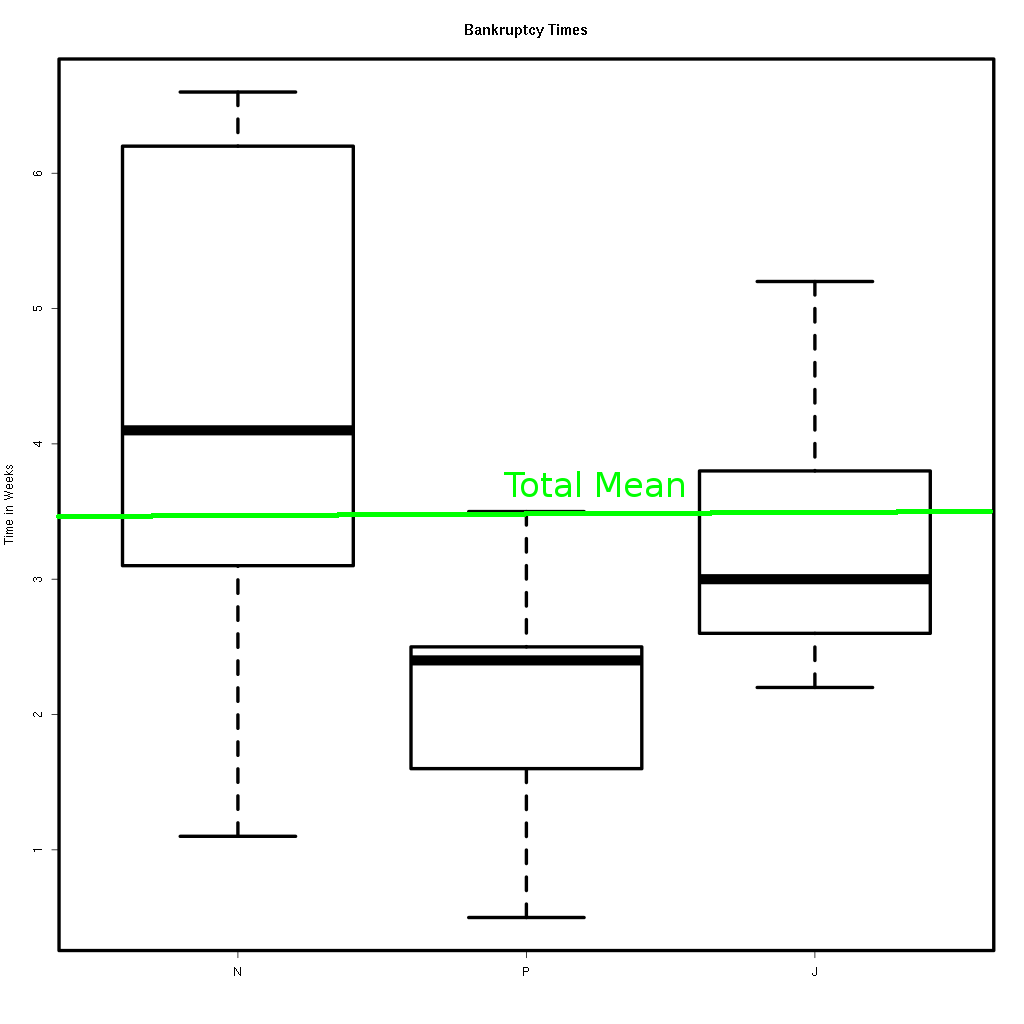
\includegraphics[width=4cm]{img/bankruptcyBoxplotTotalMean}}}
  \only<4>{\centerline{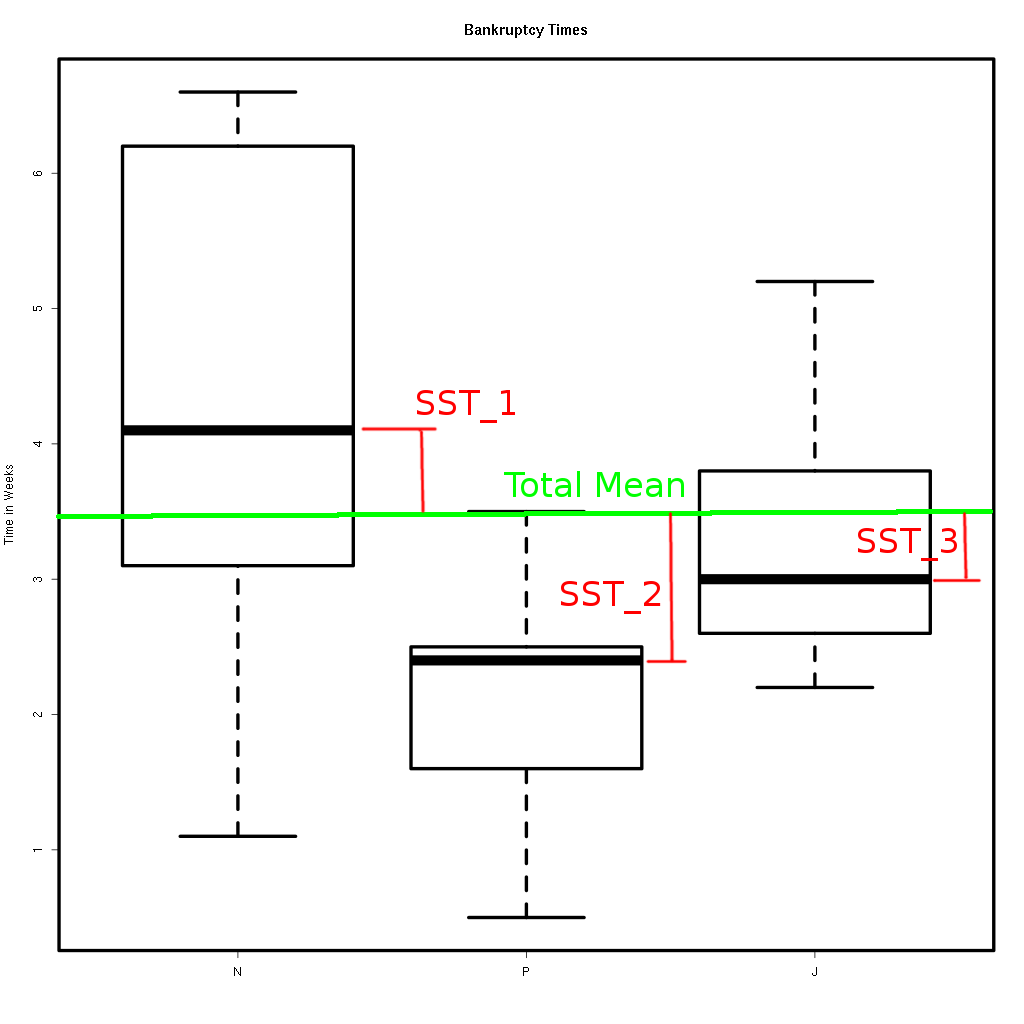
\includegraphics[width=4cm]{img/bankruptcyBoxplotSST}}}
  
\end{frame}

\begin{frame}{What Could Happen?}

  Assume the null hypothesis is true: \\
  \begin{tabular}{ll}
    SSTr small & SSE small \\
    SSTr small & SSE big \\
    SSTr big & SSE small \\
    SSTr big & SSE big \\
  \end{tabular}
  
\end{frame}

\begin{frame}{Comparing Multiple Independent Samples}

  A number of firms were sampled at random, and their plan as well as
  time in bankruptcy (in weeks) were sampled.

  \vfill
  Question: Is there a difference?


  \begin{columns}[t]
    \column{.33\textwidth}
    No Pre-Filing \\
    \begin{tabular}{l}
      1.1 \\ 6.6  \\ 3.2 \\ 5.0  \\ 6.2 \\ 3.1
    \end{tabular}
    \column{.33\textwidth}
    Pre-packaged \\
    \begin{tabular}{l}
      0.5 \\ 2.5 \\ 3.5 \\ 2.4 \\ 1.6
    \end{tabular}
    \column{.33\textwidth}
    Joint Exchange \\
    \begin{tabular}{l}
      5.2 \\ 4.1 \\ 3.5 \\ 2.2 \\ 3.0 \\ 2.3 \\ 2.9
    \end{tabular}

  \end{columns}


\end{frame}


\begin{frame}{Comparing Multiple Independent Samples}

  When a firm is in a financial crisis there are many options. One
  option is to declare some form of bankruptcy to get relief from
  creditors. There are many ways to proceed in bankruptcy. We look at
  three types of plans for getting out of bankruptcy: No Prefiling (N),
  Prepackaged (P), and Joint Exchange (J).

  \vfill

  The three measures of variance: \\
  \begin{tabular}{ll}
    SSTr & $=$ \\ % 12.04754
    SSE  & $=$ \\ % 33.98857
    SST  & $=$ \\ % 46.03611
  \end{tabular}


\end{frame}

\begin{frame}{The F Distribution}

  \begin{columns}
    \column{.5\textwidth}

    We define the following quantities:
    \begin{eqnarray*}
      MSTR & = & \frac{SSTr}{k-1}, \\    % 6.024 
      MSE  & = & \frac{SSE}{N_T - k}, \\ % 2.266
      F    & = & \frac{MSTR}{MSE}.    \\ % 2.658
    \end{eqnarray*}
    % F_cr = 3.68232

    $df_1=k-1$, and $df_2=N_T-k$.

  \vfill

    \column{.5\textwidth}

    \vfill

    \centerline{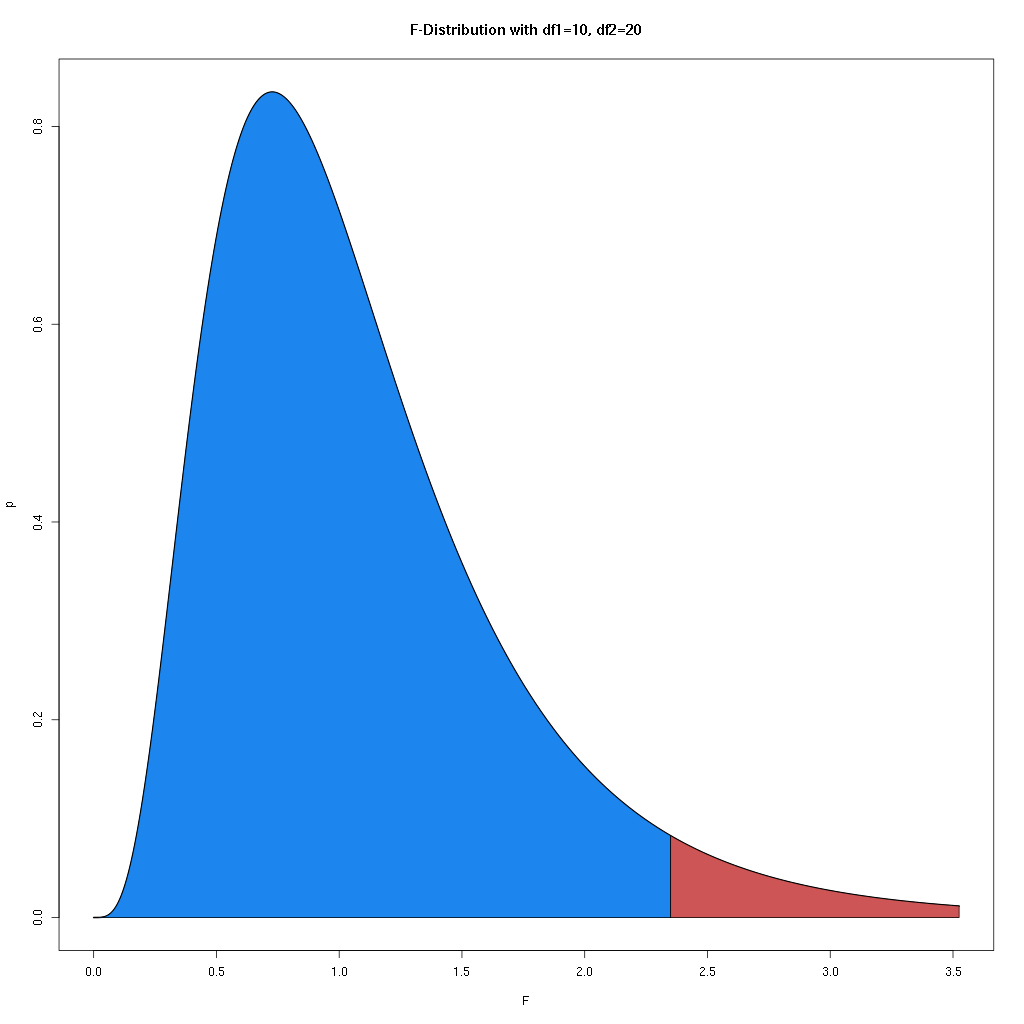
\includegraphics[width=4cm]{img/FDistribution}}

    \vfill

    \end{columns}
  
\end{frame}



\begin{frame}{F-Tables}
{\small Approximation of the critical values for the $F$-distribution for $\alpha=0.05$. }
 {
   \fontencoding{T1}
   \fontfamily{pcr}
   \fontseries{m}
   \fontshape{n}
   \fontsize{5pt}{5pt}
   \selectfont
   \begin{tabular}{l|lllllllllllll} 
     df2  & df1      1  &      2  &      3  &      4  &      5  &      6  &      7  &      8  &      9 \\ \hline 
  1 & 161.45 & 199.50 & 215.71 & 224.58 & 230.16 & 233.99 & 236.77 & 238.88 & 240.54 \\[2pt] \arrayrulecolor{light-gray}\hline\arrayrulecolor{black}  
  2 & 18.513 & 19.000 & 19.164 & 19.247 & 19.296 & 19.330 & 19.353 & 19.371 & 19.385 \\[2pt] \arrayrulecolor{light-gray}\hline\arrayrulecolor{black}  
  3 & 10.128 & 9.5521 & 9.2766 & 9.1172 & 9.0135 & 8.9406 & 8.8867 & 8.8452 & 8.8123 \\[2pt] \arrayrulecolor{light-gray}\hline\arrayrulecolor{black}  
  4 & 7.7086 & 6.9443 & 6.5914 & 6.3882 & 6.2561 & 6.1631 & 6.0942 & 6.0410 & 5.9988 \\[2pt] \arrayrulecolor{light-gray}\hline\arrayrulecolor{black}  
  5 & 6.6079 & 5.7861 & 5.4095 & 5.1922 & 5.0503 & 4.9503 & 4.8759 & 4.8183 & 4.7725 \\[2pt] \arrayrulecolor{light-gray}\hline\arrayrulecolor{black}  
  6 & 5.9874 & 5.1433 & 4.7571 & 4.5337 & 4.3874 & 4.2839 & 4.2067 & 4.1468 & 4.0990 \\[2pt] \arrayrulecolor{light-gray}\hline\arrayrulecolor{black}  
  7 & 5.5914 & 4.7374 & 4.3468 & 4.1203 & 3.9715 & 3.8660 & 3.7870 & 3.7257 & 3.6767 \\[2pt] \arrayrulecolor{light-gray}\hline\arrayrulecolor{black}  
  8 & 5.3177 & 4.4590 & 4.0662 & 3.8379 & 3.6875 & 3.5806 & 3.5005 & 3.4381 & 3.3881 \\[2pt] \arrayrulecolor{light-gray}\hline\arrayrulecolor{black}  
  9 & 5.1174 & 4.2565 & 3.8625 & 3.6331 & 3.4817 & 3.3738 & 3.2927 & 3.2296 & 3.1789 \\[2pt] \arrayrulecolor{light-gray}\hline\arrayrulecolor{black}  
 10 & 4.9646 & 4.1028 & 3.7083 & 3.4780 & 3.3258 & 3.2172 & 3.1355 & 3.0717 & 3.0204 \\[2pt] \arrayrulecolor{light-gray}\hline\arrayrulecolor{black}  
 11 & 4.8443 & 3.9823 & 3.5874 & 3.3567 & 3.2039 & 3.0946 & 3.0123 & 2.9480 & 2.8962 \\[2pt] \arrayrulecolor{light-gray}\hline\arrayrulecolor{black}  
 12 & 4.7472 & 3.8853 & 3.4903 & 3.2592 & 3.1059 & 2.9961 & 2.9134 & 2.8486 & 2.7964 \\[2pt] \arrayrulecolor{light-gray}\hline\arrayrulecolor{black}  
 13 & 4.6672 & 3.8056 & 3.4105 & 3.1791 & 3.0254 & 2.9153 & 2.8321 & 2.7669 & 2.7144 \\[2pt] \arrayrulecolor{light-gray}\hline\arrayrulecolor{black}  
 14 & 4.6001 & 3.7389 & 3.3439 & 3.1122 & 2.9582 & 2.8477 & 2.7642 & 2.6987 & 2.6458 \\[2pt] \arrayrulecolor{light-gray}\hline\arrayrulecolor{black}  
 15 & 4.5431 & 3.6823 & 3.2874 & 3.0556 & 2.9013 & 2.7905 & 2.7066 & 2.6408 & 2.5876 \\[2pt] \arrayrulecolor{light-gray}\hline\arrayrulecolor{black}  
 16 & 4.4940 & 3.6337 & 3.2389 & 3.0069 & 2.8524 & 2.7413 & 2.6572 & 2.5911 & 2.5377 \\[2pt] \arrayrulecolor{light-gray}\hline\arrayrulecolor{black}  
 17 & 4.4513 & 3.5915 & 3.1968 & 2.9647 & 2.8100 & 2.6987 & 2.6143 & 2.5480 & 2.4943 \\[2pt] \arrayrulecolor{light-gray}\hline\arrayrulecolor{black}  
 18 & 4.4139 & 3.5546 & 3.1599 & 2.9277 & 2.7729 & 2.6613 & 2.5767 & 2.5102 & 2.4563 \\[2pt] \arrayrulecolor{light-gray}\hline\arrayrulecolor{black}  
 19 & 4.3807 & 3.5219 & 3.1274 & 2.8951 & 2.7401 & 2.6283 & 2.5435 & 2.4768 & 2.4227 \\[2pt] \arrayrulecolor{light-gray}\hline\arrayrulecolor{black}  
   \end{tabular}
}
  
\end{frame}


\begin{frame}{Find the critical F for df1=4, df2=10, $\alpha=0.05$}
{\small Approximation of the critical values for the $F$-distribution for $\alpha=0.05$. }
 {
   \fontencoding{T1}
   \fontfamily{pcr}
   \fontseries{m}
   \fontshape{n}
   \fontsize{5pt}{5pt}
   \selectfont
   \begin{tabular}{l|lllllllll} 
     df2  & df1      1  &      2  &      3  &      4  &      5  &      6  &      7  &      8  &      9 \\ \hline 
  1 & 161.45 & 199.50 & 215.71 & 224.58 & 230.16 & 233.99 & 236.77 & 238.88 & 240.54 \\[2pt] \arrayrulecolor{light-gray}\hline\arrayrulecolor{black}  
  2 & 18.513 & 19.000 & 19.164 & 19.247 & 19.296 & 19.330 & 19.353 & 19.371 & 19.385 \\[2pt] \arrayrulecolor{light-gray}\hline\arrayrulecolor{black}  
  3 & 10.128 & 9.5521 & 9.2766 & 9.1172 & 9.0135 & 8.9406 & 8.8867 & 8.8452 & 8.8123 \\[2pt] \arrayrulecolor{light-gray}\hline\arrayrulecolor{black}  
  4 & 7.7086 & 6.9443 & 6.5914 & 6.3882 & 6.2561 & 6.1631 & 6.0942 & 6.0410 & 5.9988 \\[2pt] \arrayrulecolor{light-gray}\hline\arrayrulecolor{black}  
  5 & 6.6079 & 5.7861 & 5.4095 & 5.1922 & 5.0503 & 4.9503 & 4.8759 & 4.8183 & 4.7725 \\[2pt] \arrayrulecolor{light-gray}\hline\arrayrulecolor{black}  
  6 & 5.9874 & 5.1433 & 4.7571 & 4.5337 & 4.3874 & 4.2839 & 4.2067 & 4.1468 & 4.0990 \\[2pt] \arrayrulecolor{light-gray}\hline\arrayrulecolor{black}  
  7 & 5.5914 & 4.7374 & 4.3468 & 4.1203 & 3.9715 & 3.8660 & 3.7870 & 3.7257 & 3.6767 \\[2pt] \arrayrulecolor{light-gray}\hline\arrayrulecolor{black}  
  8 & 5.3177 & 4.4590 & 4.0662 & 3.8379 & 3.6875 & 3.5806 & 3.5005 & 3.4381 & 3.3881 \\[2pt] \arrayrulecolor{light-gray}\hline\arrayrulecolor{black}  
  9 & 5.1174 & 4.2565 & 3.8625 & 3.6331 & 3.4817 & 3.3738 & 3.2927 & 3.2296 & 3.1789 \\[2pt] \arrayrulecolor{light-gray}\hline\arrayrulecolor{black}  
 10 & 4.9646 & 4.1028 & 3.7083 & 3.4780 & 3.3258 & 3.2172 & 3.1355 & 3.0717 & 3.0204 \\[2pt] \arrayrulecolor{light-gray}\hline\arrayrulecolor{black}  
 11 & 4.8443 & 3.9823 & 3.5874 & 3.3567 & 3.2039 & 3.0946 & 3.0123 & 2.9480 & 2.8962 \\[2pt] \arrayrulecolor{light-gray}\hline\arrayrulecolor{black}  
 12 & 4.7472 & 3.8853 & 3.4903 & 3.2592 & 3.1059 & 2.9961 & 2.9134 & 2.8486 & 2.7964 \\[2pt] \arrayrulecolor{light-gray}\hline\arrayrulecolor{black}  
 13 & 4.6672 & 3.8056 & 3.4105 & 3.1791 & 3.0254 & 2.9153 & 2.8321 & 2.7669 & 2.7144 \\[2pt] \arrayrulecolor{light-gray}\hline\arrayrulecolor{black}  
 14 & 4.6001 & 3.7389 & 3.3439 & 3.1122 & 2.9582 & 2.8477 & 2.7642 & 2.6987 & 2.6458 \\[2pt] \arrayrulecolor{light-gray}\hline\arrayrulecolor{black}  
 15 & 4.5431 & 3.6823 & 3.2874 & 3.0556 & 2.9013 & 2.7905 & 2.7066 & 2.6408 & 2.5876 \\[2pt] \arrayrulecolor{light-gray}\hline\arrayrulecolor{black}  
 16 & 4.4940 & 3.6337 & 3.2389 & 3.0069 & 2.8524 & 2.7413 & 2.6572 & 2.5911 & 2.5377 \\[2pt] \arrayrulecolor{light-gray}\hline\arrayrulecolor{black}  
 17 & 4.4513 & 3.5915 & 3.1968 & 2.9647 & 2.8100 & 2.6987 & 2.6143 & 2.5480 & 2.4943 \\[2pt] \arrayrulecolor{light-gray}\hline\arrayrulecolor{black}  
 18 & 4.4139 & 3.5546 & 3.1599 & 2.9277 & 2.7729 & 2.6613 & 2.5767 & 2.5102 & 2.4563 \\[2pt] \arrayrulecolor{light-gray}\hline\arrayrulecolor{black}  
 19 & 4.3807 & 3.5219 & 3.1274 & 2.8951 & 2.7401 & 2.6283 & 2.5435 & 2.4768 & 2.4227 \\[2pt] \arrayrulecolor{light-gray}\hline\arrayrulecolor{black}  
   \end{tabular}
}
  
\end{frame}


\begin{frame}{Find the critical F for df1=4, df2=10, $\alpha=0.05$}
{\small Approximation of the critical values for the $F$-distribution for $\alpha=0.05$. }
 {
   \fontencoding{T1}
   \fontfamily{pcr}
   \fontseries{m}
   \fontshape{n}
   \fontsize{5pt}{5pt}
   \selectfont
   \begin{tabular}{l|lll>{\columncolor{light-blue}}llllll} 
     df2  & df1      1  &      2  &      3  &      4  &      5  &      6  &      7  &      8  &      9 \\ \hline 
  1 & 161.45 & 199.50 & 215.71 & 224.58 & 230.16 & 233.99 & 236.77 & 238.88 & 240.54 \\[2pt] \arrayrulecolor{light-gray}\hline\arrayrulecolor{black}  
  2 & 18.513 & 19.000 & 19.164 & 19.247 & 19.296 & 19.330 & 19.353 & 19.371 & 19.385 \\[2pt] \arrayrulecolor{light-gray}\hline\arrayrulecolor{black}  
  3 & 10.128 & 9.5521 & 9.2766 & 9.1172 & 9.0135 & 8.9406 & 8.8867 & 8.8452 & 8.8123 \\[2pt] \arrayrulecolor{light-gray}\hline\arrayrulecolor{black}  
  4 & 7.7086 & 6.9443 & 6.5914 & 6.3882 & 6.2561 & 6.1631 & 6.0942 & 6.0410 & 5.9988 \\[2pt] \arrayrulecolor{light-gray}\hline\arrayrulecolor{black}  
  5 & 6.6079 & 5.7861 & 5.4095 & 5.1922 & 5.0503 & 4.9503 & 4.8759 & 4.8183 & 4.7725 \\[2pt] \arrayrulecolor{light-gray}\hline\arrayrulecolor{black}  
  6 & 5.9874 & 5.1433 & 4.7571 & 4.5337 & 4.3874 & 4.2839 & 4.2067 & 4.1468 & 4.0990 \\[2pt] \arrayrulecolor{light-gray}\hline\arrayrulecolor{black}  
  7 & 5.5914 & 4.7374 & 4.3468 & 4.1203 & 3.9715 & 3.8660 & 3.7870 & 3.7257 & 3.6767 \\[2pt] \arrayrulecolor{light-gray}\hline\arrayrulecolor{black}  
  8 & 5.3177 & 4.4590 & 4.0662 & 3.8379 & 3.6875 & 3.5806 & 3.5005 & 3.4381 & 3.3881 \\[2pt] \arrayrulecolor{light-gray}\hline\arrayrulecolor{black}  
  9 & 5.1174 & 4.2565 & 3.8625 & 3.6331 & 3.4817 & 3.3738 & 3.2927 & 3.2296 & 3.1789 \\[2pt] \arrayrulecolor{light-gray}\hline\arrayrulecolor{black}  
 10 & 4.9646 & 4.1028 & 3.7083 & 3.4780 & 3.3258 & 3.2172 & 3.1355 & 3.0717 & 3.0204 \\[2pt] \arrayrulecolor{light-gray}\hline\arrayrulecolor{black}  
 11 & 4.8443 & 3.9823 & 3.5874 & 3.3567 & 3.2039 & 3.0946 & 3.0123 & 2.9480 & 2.8962 \\[2pt] \arrayrulecolor{light-gray}\hline\arrayrulecolor{black}  
 12 & 4.7472 & 3.8853 & 3.4903 & 3.2592 & 3.1059 & 2.9961 & 2.9134 & 2.8486 & 2.7964 \\[2pt] \arrayrulecolor{light-gray}\hline\arrayrulecolor{black}  
 13 & 4.6672 & 3.8056 & 3.4105 & 3.1791 & 3.0254 & 2.9153 & 2.8321 & 2.7669 & 2.7144 \\[2pt] \arrayrulecolor{light-gray}\hline\arrayrulecolor{black}  
 14 & 4.6001 & 3.7389 & 3.3439 & 3.1122 & 2.9582 & 2.8477 & 2.7642 & 2.6987 & 2.6458 \\[2pt] \arrayrulecolor{light-gray}\hline\arrayrulecolor{black}  
 15 & 4.5431 & 3.6823 & 3.2874 & 3.0556 & 2.9013 & 2.7905 & 2.7066 & 2.6408 & 2.5876 \\[2pt] \arrayrulecolor{light-gray}\hline\arrayrulecolor{black}  
 16 & 4.4940 & 3.6337 & 3.2389 & 3.0069 & 2.8524 & 2.7413 & 2.6572 & 2.5911 & 2.5377 \\[2pt] \arrayrulecolor{light-gray}\hline\arrayrulecolor{black}  
 17 & 4.4513 & 3.5915 & 3.1968 & 2.9647 & 2.8100 & 2.6987 & 2.6143 & 2.5480 & 2.4943 \\[2pt] \arrayrulecolor{light-gray}\hline\arrayrulecolor{black}  
 18 & 4.4139 & 3.5546 & 3.1599 & 2.9277 & 2.7729 & 2.6613 & 2.5767 & 2.5102 & 2.4563 \\[2pt] \arrayrulecolor{light-gray}\hline\arrayrulecolor{black}  
 19 & 4.3807 & 3.5219 & 3.1274 & 2.8951 & 2.7401 & 2.6283 & 2.5435 & 2.4768 & 2.4227 \\[2pt] \arrayrulecolor{light-gray}\hline\arrayrulecolor{black}  
   \end{tabular}
}
  
\end{frame}

\begin{frame}{Find the critical F for df1=4, df2=10, $\alpha=0.05$}
{\small Approximation of the critical values for the $F$-distribution for $\alpha=0.05$. }
 {
   \fontencoding{T1}
   \fontfamily{pcr}
   \fontseries{m}
   \fontshape{n}
   \fontsize{5pt}{5pt}
   \selectfont
   \begin{tabular}{l|lll>{\columncolor{light-blue}}llllll} 
     df2  & df1      1  &      2  &      3  &      4  &      5  &      6  &      7  &      8  &      9 \\ \hline 
  1 & 161.45 & 199.50 & 215.71 & 224.58 & 230.16 & 233.99 & 236.77 & 238.88 & 240.54 \\[2pt] \arrayrulecolor{light-gray}\hline\arrayrulecolor{black}  
  2 & 18.513 & 19.000 & 19.164 & 19.247 & 19.296 & 19.330 & 19.353 & 19.371 & 19.385 \\[2pt] \arrayrulecolor{light-gray}\hline\arrayrulecolor{black}  
  3 & 10.128 & 9.5521 & 9.2766 & 9.1172 & 9.0135 & 8.9406 & 8.8867 & 8.8452 & 8.8123 \\[2pt] \arrayrulecolor{light-gray}\hline\arrayrulecolor{black}  
  4 & 7.7086 & 6.9443 & 6.5914 & 6.3882 & 6.2561 & 6.1631 & 6.0942 & 6.0410 & 5.9988 \\[2pt] \arrayrulecolor{light-gray}\hline\arrayrulecolor{black}  
  5 & 6.6079 & 5.7861 & 5.4095 & 5.1922 & 5.0503 & 4.9503 & 4.8759 & 4.8183 & 4.7725 \\[2pt] \arrayrulecolor{light-gray}\hline\arrayrulecolor{black}  
  6 & 5.9874 & 5.1433 & 4.7571 & 4.5337 & 4.3874 & 4.2839 & 4.2067 & 4.1468 & 4.0990 \\[2pt] \arrayrulecolor{light-gray}\hline\arrayrulecolor{black}  
  7 & 5.5914 & 4.7374 & 4.3468 & 4.1203 & 3.9715 & 3.8660 & 3.7870 & 3.7257 & 3.6767 \\[2pt] \arrayrulecolor{light-gray}\hline\arrayrulecolor{black}  
  8 & 5.3177 & 4.4590 & 4.0662 & 3.8379 & 3.6875 & 3.5806 & 3.5005 & 3.4381 & 3.3881 \\[2pt] \arrayrulecolor{light-gray}\hline\arrayrulecolor{black}  
  9 & 5.1174 & 4.2565 & 3.8625 & 3.6331 & 3.4817 & 3.3738 & 3.2927 & 3.2296 & 3.1789 \\[2pt] \arrayrulecolor{light-gray}\hline\arrayrulecolor{black}  
\rowcolor{light-red} 10 & 4.9646 & 4.1028 & 3.7083 & 3.4780 & 3.3258 & 3.2172 & 3.1355 & 3.0717 & 3.0204 \\[2pt] \arrayrulecolor{light-gray}\hline\arrayrulecolor{black}  
 11 & 4.8443 & 3.9823 & 3.5874 & 3.3567 & 3.2039 & 3.0946 & 3.0123 & 2.9480 & 2.8962 \\[2pt] \arrayrulecolor{light-gray}\hline\arrayrulecolor{black}  
 12 & 4.7472 & 3.8853 & 3.4903 & 3.2592 & 3.1059 & 2.9961 & 2.9134 & 2.8486 & 2.7964 \\[2pt] \arrayrulecolor{light-gray}\hline\arrayrulecolor{black}  
 13 & 4.6672 & 3.8056 & 3.4105 & 3.1791 & 3.0254 & 2.9153 & 2.8321 & 2.7669 & 2.7144 \\[2pt] \arrayrulecolor{light-gray}\hline\arrayrulecolor{black}  
 14 & 4.6001 & 3.7389 & 3.3439 & 3.1122 & 2.9582 & 2.8477 & 2.7642 & 2.6987 & 2.6458 \\[2pt] \arrayrulecolor{light-gray}\hline\arrayrulecolor{black}  
 15 & 4.5431 & 3.6823 & 3.2874 & 3.0556 & 2.9013 & 2.7905 & 2.7066 & 2.6408 & 2.5876 \\[2pt] \arrayrulecolor{light-gray}\hline\arrayrulecolor{black}  
 16 & 4.4940 & 3.6337 & 3.2389 & 3.0069 & 2.8524 & 2.7413 & 2.6572 & 2.5911 & 2.5377 \\[2pt] \arrayrulecolor{light-gray}\hline\arrayrulecolor{black}  
 17 & 4.4513 & 3.5915 & 3.1968 & 2.9647 & 2.8100 & 2.6987 & 2.6143 & 2.5480 & 2.4943 \\[2pt] \arrayrulecolor{light-gray}\hline\arrayrulecolor{black}  
 18 & 4.4139 & 3.5546 & 3.1599 & 2.9277 & 2.7729 & 2.6613 & 2.5767 & 2.5102 & 2.4563 \\[2pt] \arrayrulecolor{light-gray}\hline\arrayrulecolor{black}  
 19 & 4.3807 & 3.5219 & 3.1274 & 2.8951 & 2.7401 & 2.6283 & 2.5435 & 2.4768 & 2.4227 \\[2pt] \arrayrulecolor{light-gray}\hline\arrayrulecolor{black}  
   \end{tabular}
}
  
\end{frame}


\begin{frame}{Clicker Quiz}
  \iftoggle{clicker}{%
    \redText{\textbf{Determine the Critical F for $\alpha=0.05$, $df1=2$, and $df2=15$.}}
  }

{\small Approximation of the critical values for the $F$-distribution for $\alpha=0.05$. }
 {
   \fontencoding{T1}
   \fontfamily{pcr}
   \fontseries{m}
   \fontshape{n}
   \fontsize{5pt}{5pt}
   \selectfont
   \begin{tabular}{l|lllllllllllll} 
     df2  & df1      1  &      2  &      3  &      4  &      5  &      6  &      7  &      8  &      9 \\ \hline 
  1 & 161.45 & 199.50 & 215.71 & 224.58 & 230.16 & 233.99 & 236.77 & 238.88 & 240.54 \\[2pt] \arrayrulecolor{light-gray}\hline\arrayrulecolor{black}  
  2 & 18.513 & 19.000 & 19.164 & 19.247 & 19.296 & 19.330 & 19.353 & 19.371 & 19.385 \\[2pt] \arrayrulecolor{light-gray}\hline\arrayrulecolor{black}  
  3 & 10.128 & 9.5521 & 9.2766 & 9.1172 & 9.0135 & 8.9406 & 8.8867 & 8.8452 & 8.8123 \\[2pt] \arrayrulecolor{light-gray}\hline\arrayrulecolor{black}  
  4 & 7.7086 & 6.9443 & 6.5914 & 6.3882 & 6.2561 & 6.1631 & 6.0942 & 6.0410 & 5.9988 \\[2pt] \arrayrulecolor{light-gray}\hline\arrayrulecolor{black}  
  5 & 6.6079 & 5.7861 & 5.4095 & 5.1922 & 5.0503 & 4.9503 & 4.8759 & 4.8183 & 4.7725 \\[2pt] \arrayrulecolor{light-gray}\hline\arrayrulecolor{black}  
  6 & 5.9874 & 5.1433 & 4.7571 & 4.5337 & 4.3874 & 4.2839 & 4.2067 & 4.1468 & 4.0990 \\[2pt] \arrayrulecolor{light-gray}\hline\arrayrulecolor{black}  
  7 & 5.5914 & 4.7374 & 4.3468 & 4.1203 & 3.9715 & 3.8660 & 3.7870 & 3.7257 & 3.6767 \\[2pt] \arrayrulecolor{light-gray}\hline\arrayrulecolor{black}  
  8 & 5.3177 & 4.4590 & 4.0662 & 3.8379 & 3.6875 & 3.5806 & 3.5005 & 3.4381 & 3.3881 \\[2pt] \arrayrulecolor{light-gray}\hline\arrayrulecolor{black}  
  9 & 5.1174 & 4.2565 & 3.8625 & 3.6331 & 3.4817 & 3.3738 & 3.2927 & 3.2296 & 3.1789 \\[2pt] \arrayrulecolor{light-gray}\hline\arrayrulecolor{black}  
 10 & 4.9646 & 4.1028 & 3.7083 & 3.4780 & 3.3258 & 3.2172 & 3.1355 & 3.0717 & 3.0204 \\[2pt] \arrayrulecolor{light-gray}\hline\arrayrulecolor{black}  
 11 & 4.8443 & 3.9823 & 3.5874 & 3.3567 & 3.2039 & 3.0946 & 3.0123 & 2.9480 & 2.8962 \\[2pt] \arrayrulecolor{light-gray}\hline\arrayrulecolor{black}  
 12 & 4.7472 & 3.8853 & 3.4903 & 3.2592 & 3.1059 & 2.9961 & 2.9134 & 2.8486 & 2.7964 \\[2pt] \arrayrulecolor{light-gray}\hline\arrayrulecolor{black}  
 13 & 4.6672 & 3.8056 & 3.4105 & 3.1791 & 3.0254 & 2.9153 & 2.8321 & 2.7669 & 2.7144 \\[2pt] \arrayrulecolor{light-gray}\hline\arrayrulecolor{black}  
 14 & 4.6001 & 3.7389 & 3.3439 & 3.1122 & 2.9582 & 2.8477 & 2.7642 & 2.6987 & 2.6458 \\[2pt] \arrayrulecolor{light-gray}\hline\arrayrulecolor{black}  
 15 & 4.5431 & 3.6823 & 3.2874 & 3.0556 & 2.9013 & 2.7905 & 2.7066 & 2.6408 & 2.5876 \\[2pt] \arrayrulecolor{light-gray}\hline\arrayrulecolor{black}  
 16 & 4.4940 & 3.6337 & 3.2389 & 3.0069 & 2.8524 & 2.7413 & 2.6572 & 2.5911 & 2.5377 \\[2pt] \arrayrulecolor{light-gray}\hline\arrayrulecolor{black}  
 17 & 4.4513 & 3.5915 & 3.1968 & 2.9647 & 2.8100 & 2.6987 & 2.6143 & 2.5480 & 2.4943 \\[2pt] \arrayrulecolor{light-gray}\hline\arrayrulecolor{black}  
 18 & 4.4139 & 3.5546 & 3.1599 & 2.9277 & 2.7729 & 2.6613 & 2.5767 & 2.5102 & 2.4563 \\[2pt] \arrayrulecolor{light-gray}\hline\arrayrulecolor{black}  
 19 & 4.3807 & 3.5219 & 3.1274 & 2.8951 & 2.7401 & 2.6283 & 2.5435 & 2.4768 & 2.4227 \\[2pt] \arrayrulecolor{light-gray}\hline\arrayrulecolor{black}  
   \end{tabular}
}

    \iftoggle{clicker}{%

      \vfill

      \begin{tabular}{l@{\hspace{3em}}l@{\hspace{3em}}l@{\hspace{3em}}l}
        \redText{A: 3.2874}  & \redText{B: 3.6823} & \redText{C: 3.7389}
      \end{tabular}

    }

  
\end{frame}

\subsection{Results and Conclusions}

\begin{frame}{The F Statistic for the Time in Bankruptcy}

  \begin{columns}
    \column{.5\textwidth}

    We define the following quantities:
    \begin{eqnarray*}
      MSTR  & = & \frac{SSTr}{k-1}, \\
      MSE   & = & \frac{SSE}{N_T - k}, \\
      F*    & = & \frac{MSTR}{MSE}, \\
      F_{cr} & \approx &
    \end{eqnarray*}

    \vfill

    \column{.5\textwidth}

    \vfill

    \centerline{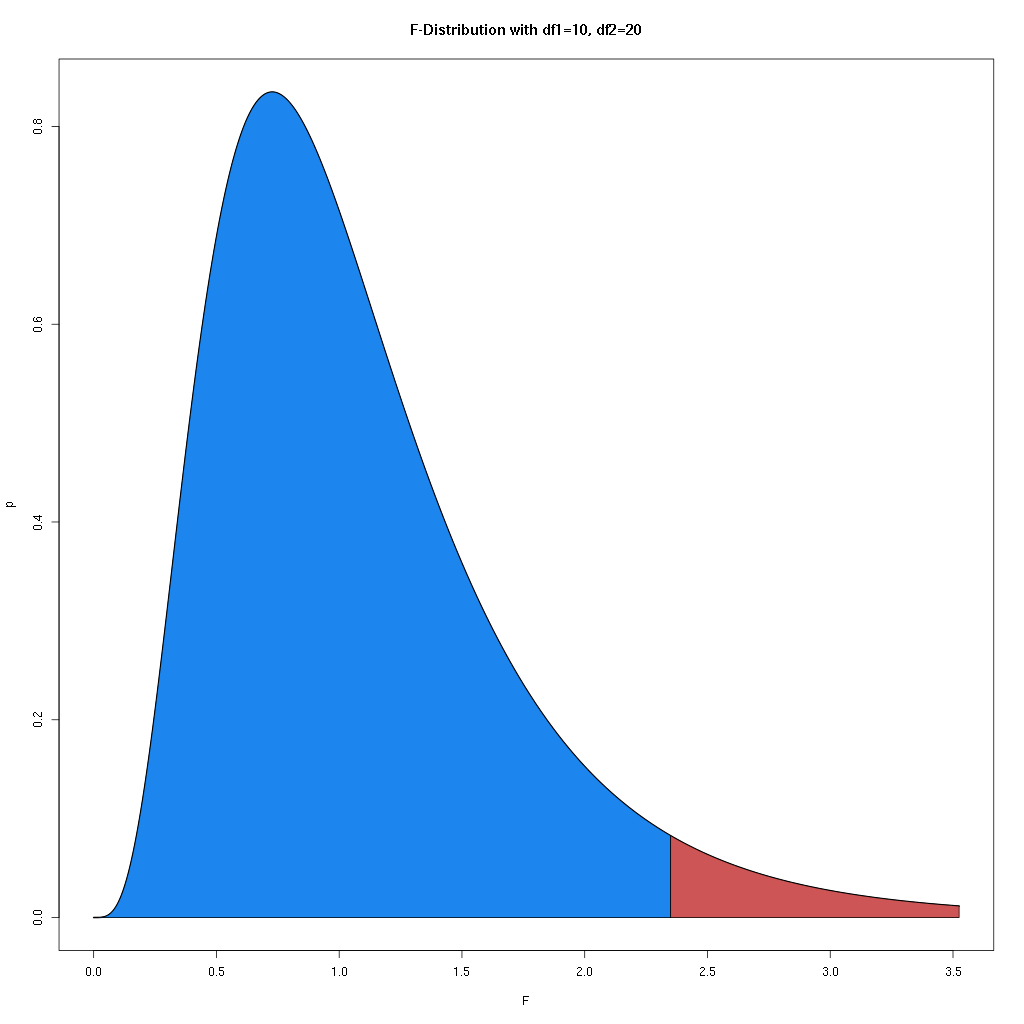
\includegraphics[width=4cm]{img/FDistribution}}

    \vfill

    \end{columns}

    \uncover<2->{%

      We cannot reject $H_0$ with a confidence level of 95\% and using an F distribution with df1=2 and df2=15.

    }
  
\end{frame}



\begin{frame}[fragile]{One Last Note}

  Nobody does this nonsense by hand! (Except, of course, the poor
  schmucks who take introductory statistics courses.)

  \vfill

  What we do in practice:

 {
   \fontencoding{T1}
   \fontfamily{pcr}
   \fontseries{m}
   \fontshape{n}
   \fontsize{5pt}{5pt}
   \selectfont

\begin{verbatim}
> bankruptcyTime <- read.csv('bankruptcy.csv')
> comparison <- aov(bankruptcyTime$t ~ bankruptcyTime$type)
> comparison
Call:
   aov(formula = bankruptcyTime$t ~ bankruptcyTime$type)

Terms:
                bankruptcyTime$type Residuals
Sum of Squares             12.04754  33.98857
Deg. of Freedom                   2        15

Residual standard error: 1.505292
Estimated effects may be unbalanced
> summary(comparison)
                    Df Sum Sq Mean Sq F value Pr(>F)
bankruptcyTime$type  2  12.05   6.024   2.658  0.103
Residuals           15  33.99   2.266               
>
\end{verbatim}
}
 
\redText{You need to know how to read this information!}

 
\end{frame}

%%% Local Variables: 
%%% mode: latex
%%% TeX-master: t
%%% End: 
